%using the old elsarticle cls by Elsevier
\documentclass[preprint,12pt,3p]{elsarticle}

%% Use the option review to obtain double line spacing
%% \documentclass[preprint,review,12pt]{elsarticle}

%% Use the options 1p,twocolumn; 3p; 3p,twocolumn; 5p; or 5p,twocolumn
%% for a journal layout:
%% \documentclass[final,1p,times]{elsarticle}
%% \documentclass[final,1p,times,twocolumn]{elsarticle}
%% \documentclass[final,3p,times]{elsarticle}
%% \documentclass[final,3p,times,twocolumn]{elsarticle}
%% \documentclass[final,5p,times]{elsarticle}
%% \documentclass[final,5p,times,twocolumn]{elsarticle}

%% if you use PostScript figures in your article
%% use the graphics package for simple commands
%% \usepackage{graphics}
%% or use the graphicx package for more complicated commands
%% \usepackage{graphicx}
%% or use the epsfig package if you prefer to use the old commands
%% \usepackage{epsfig}

%% The amssymb package provides various useful mathematical symbols
\usepackage{amssymb}
%% The amsthm package provides extended theorem environments
%% \usepackage{amsthm}
\usepackage{amssymb,amsmath}
%% The lineno packages adds line numbers. Start line numbering with
%% \begin{linenumbers}, end it with \end{linenumbers}. Or switch it on
%% for the whole article with \linenumbers after \end{frontmatter}.
%% \usepackage{lineno}

%% natbib.sty is loaded by default. However, natbib options can be
%% provided with \biboptions{...} command. Following options are
%% valid:

%%   round  -  round parentheses are used (default)
%%   square -  square brackets are used   [option]
%%   curly  -  curly braces are used      {option}
%%   angle  -  angle brackets are used    <option>
%%   semicolon  -  multiple citations separated by semi-colon
%%   colon  - same as semicolon, an earlier confusion
%%   comma  -  separated by comma
%%   numbers-  selects numerical citations
%%   super  -  numerical citations as superscripts
%%   sort   -  sorts multiple citations according to order in ref. list
%%   sort&compress   -  like sort, but also compresses numerical citations
%%   compress - compresses without sorting
%%
%% \biboptions{comma,round}

% \biboptions{}


%\journal{Nuclear Physics B}
%journal{Numerical Practice Reports}
Numerical Practice Reports
\begin{document}

\begin{frontmatter}

\title{ \texttt{Numerical Practice 2 }}
%\tnotetext[label0]{This is only an example}


\author{Aakash Patil}
\address{aakash.patil@master.centralelille.fr}

%\ead[url]{author-one-homepage.com}

\begin{abstract}
1. Study of Tridiagonal matrix Method.  
\\
2. Study of error as a function of number of discretization points.
\end{abstract}

%\begin{keyword}
%% keywords here, in the form: keyword \sep keyword
%example \sep \LaTeX \sep template
%% MSC codes here, in the form: \MSC code \sep code
%% or \MSC[2008] code \sep code (2000 is the default)
%\end{keyword}

\end{frontmatter}

%%
%% Start line numbering here if you want
%%
% \linenumbers

%% main text
\section{Tridiagonal Matrix}
%\label{sec1}
A tridiagonal matrix is a sparse matrix that has nonzero elements only on the main diagonal, the first diagonal below this, and the first diagonal above the main diagonal. This means that such matrices all have 0s at the same known positions. For instance, the only nonzero elements are either on the diagonal or on subdiagonals just below or above the diagonal, and all other elements are guaranteed to be 0, such as for a $n\times n$ tridiagonal matrix
$$
A = \left[
  \begin{array}{ccccc}
    a & b    & 0    &\cdots& 0\\
    c & a    & b    & &\vdots\\
    0 &\ddots&\ddots&\ddots& 0\\
    \vdots&   & c    & a & b\\
    0 & \cdots& 0    & c & a
  \end{array}
  \right]
$$


\section{Tridiagonal Matrix Algorithm}
In numerical linear algebra, the tridiagonal matrix algorithm, also known as the Thomas
algorithm (named after Llewellyn Thomas), is a
simplified form of Gaussian elimination
that can be used to solve tridiagonal systems
of equations. A tridiagonal system for \emph{n} unknowns may be written
as

\[a_i x_{i - 1}  + b_i x_i  + c_i x_{i + 1}  = d_i , \,\!\] where
\(a_1  = 0\,\) and \(c_n = 0\,\).

\[\begin{bmatrix}
   {b_1} & {c_1} & {   } & {   } & { 0 } \\
   {a_2} & {b_2} & {c_2} & {   } & {   } \\
   {   } & {a_3} & {b_3} & \ddots & {   } \\
   {   } & {   } & \ddots & \ddots & {c_{n-1}}\\
   { 0 } & {   } & {   } & {a_n} & {b_n}\\
\end{bmatrix}
\begin{bmatrix}
   {x_1 }  \\
   {x_2 }  \\
   {x_3 }  \\
   \vdots   \\
   {x_n }  \\
\end{bmatrix}
=
\begin{bmatrix}
   {d_1 }  \\
   {d_2 }  \\
   {d_3 }  \\
   \vdots   \\
   {d_n }  \\
\end{bmatrix}
.\]

For such systems, the solution can be obtained in \(O(n)\) operations
instead of \(O(n^3)\) required by Gaussian
elimination. A first sweep eliminates the \(a_i\)'s, and then an
(abbreviated) backward substitution produces the solution. Examples of
such matrices commonly arise from the discretization of 1D
Poisson equation; similar systems of
matrices also arise in the nearest neighbor effect models.

Thomas' algorithm is not numerically stable in general,
but is so in several special cases, such as when the matrix is
diagonally dominant(either by rows or
columns) or symmetric positive
definite. If
stability is required in the general case, Gaussian elimination with
partial pivoting is recommended
instead.

\subsection{Method}\label{method}

The forward sweep consists of modifying the coefficients as follows,
denoting the new coefficients with primes:

\[c'_i =
\begin{cases}
\begin{array}{lcl}
  \cfrac{c_i}{b_i}                  & ; & i = 1 \\
  \cfrac{c_i}{b_i - a_i c'_{i - 1}} & ; & i = 2, 3, \dots, n-1 \\
\end{array}
\end{cases}
\,\]

and

\[d'_i =
\begin{cases}
\begin{array}{lcl}
  \cfrac{d_i}{b_i}                  & ; & i = 1 \\
  \cfrac{d_i - a_i d'_{i - 1}}{b_i - a_i c'_{i - 1}} & ; & i = 2, 3, \dots, n. \\
\end{array}
\end{cases}
\,\]

The solution is then obtained by back substitution:

\[x_n = d'_n\,\]

\[x_i = d'_i - c'_i x_{i + 1} \qquad ; \ i = n - 1, n - 2, \ldots, 1.\]

\subsection{Derivation}\label{derivation}

The derivation of the tridiagonal matrix algorithm is a special case of Gaussian elimination.

Suppose that the unknowns are \(x_1,\ldots, x_n\), and that the
equations to be solved are:

\[\begin{align}
b_1 x_1 + c_1 x_2 & = d_1;& i & = 1 \\
a_i x_{i - 1} + b_i x_i  + c_i x_{i + 1} & = d_i;& i & = 2, \ldots, n - 1 \\
a_n x_{n - 1} + b_n x_n & = d_n;& i & = n.
\end{align}\]

Consider modifying the second (\(i = 2\)) equation with the first
equation as follows:

\[(\mbox{equation 2}) \cdot b_1 - (\mbox{equation 1}) \cdot a_2\]

which would give:

\[(a_2 x_1 + b_2 x_2  + c_2 x_3) b_1 - (b_1 x_1  + c_1 x_2) a_2 = d_2 b_1 - d_1 a_2
\,\]

\[(b_2 b_1 - c_1 a_2) x_2  + c_2 b_1 x_3 = d_2 b_1 - d_1 a_2
\,\]

where the second equation immediately above is a simplified version of
the equation immediately preceding it. The effect is that \(x_1\) has
been eliminated from the second equation. Using a similar tactic with
the modified second equation on the third equation yields:

\[(a_3 x_2 + b_3 x_3 + c_3 x_4) (b_2 b_1 - c_1 a_2) -
((b_2 b_1 - c_1 a_2) x_2 + c_2 b_1 x_3) a_3
= d_3 (b_2 b_1 - c_1 a_2) - (d_2 b_1 - d_1 a_2) a_3
\,\]

\[(b_3 (b_2 b_1 - c_1 a_2) - c_2 b_1 a_3 )x_3 + c_3 (b_2 b_1 - c_1 a_2) x_4
= d_3 (b_2 b_1 - c_1 a_2) - (d_2 b_1 - d_1 a_2) a_3.
\,\]

This time \(x_2\) was eliminated. If this procedure is repeated until
the \(n^{th}\) row; the (modified) \(n^{th}\) equation will involve only
one unknown, \(x_n\). This may be solved for and then used to solve the
\((n - 1)^{th}\) equation, and so on until all of the unknowns are
solved for.

Clearly, the coefficients on the modified equations get more and more
complicated if stated explicitly. By examining the procedure, the
modified coefficients (notated with tildes) may instead be defined
recursively:

\[\tilde a_i = 0\,\]

\[\tilde b_1 = b_1\,\]

\[\tilde b_i = b_i \tilde b_{i - 1} - \tilde c_{i - 1} a_i\,\]

\[\tilde c_1 = c_1\,\]

\[\tilde c_i = c_i \tilde b_{i - 1}\,\]

\[\tilde d_1 = d_1\,\]

\[\tilde d_i = d_i \tilde b_{i - 1} - \tilde d_{i - 1} a_i.\,\]

To further hasten the solution process, \(\tilde b_i\) may be divided
out (if there's no division by zero risk), the newer modified
coefficients, each notated with a prime, will be:

\[a'_i = 0\,\]

\[b'_i = 1\,\]

\[c'_1 = \frac{c_1}{b_1}\,\]

\[c'_i = \frac{c_i}{b_i - c'_{i - 1} a_i}\,\]

\[d'_1 = \frac{d_1}{b_1}\,\]

\[d'_i = \frac{d_i - d'_{i - 1} a_i}{b_i - c'_{i - 1} a_i}.\,\]

This gives the following system with the same unknowns and coefficients
defined in terms of the original ones above:

\[\begin{array}{lcl}
x_i + c'_i x_{i + 1} = d'_i \qquad &;& \ i = 1, \ldots, n - 1 \\
x_n = d'_n \qquad &;& \ i = n. \\
\end{array}
\,\]

The last equation involves only one unknown. Solving it in turn reduces
the next last equation to one unknown, so that this backward
substitution can be used to find all of the unknowns:

\[x_n = d'_n\,\]

\[x_i = d'_i - c'_i x_{i + 1} \qquad ; \ i = n - 1, n - 2, \ldots, 1.\]



\section{Code}

Random numbers were used to find the error. Firstly, $xRand$ of size $n \times 1$ was generated using random numbers. Then, $d$ was computed as $d=matmul(A,xRand)$ using the given $A$ of size $n \times n$ and the $xRand$ of size $n \times 1$ generated using random numbers. Later, the function to solve tridiagonal matrix was called by supplying $A$ and the previous $d$ to obtain the numerical value of $x$. 

The code has been uploaded to \\
https://github.com/aakash30jan/ClassWork-TurbulenceMaster/tree/master/11-11-2017/src/
\newpage
\section{Results}


\subsection{Plots}
 \begin{figure}[!htbp]
\centering
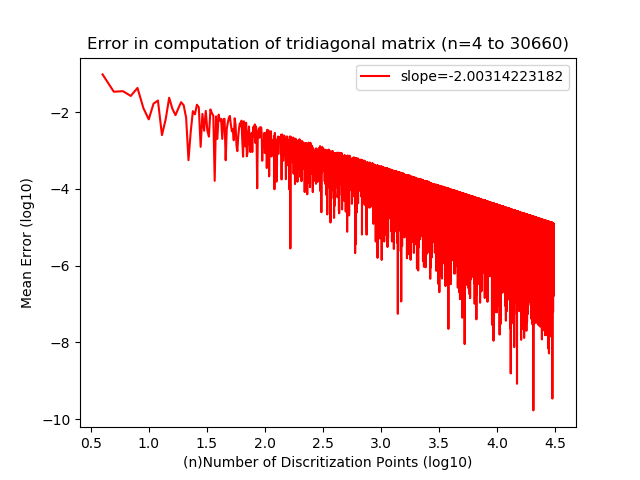
\includegraphics[width=0.7\linewidth]{data1_NPlog.png}
\caption{Normal scale with log computed plot of error in numerical computation of tridiagonal matrix (N=4 to 30660 with step of 1)}
\label{fig:data1_NPlog}
\end{figure}


 \begin{figure}[!htbp]
\centering
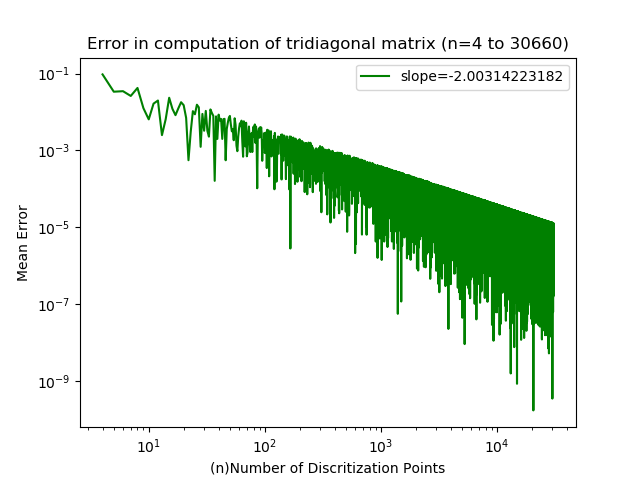
\includegraphics[width=0.7\linewidth]{data1_PLlog.png}
\caption{Log scale plot of error in numerical computation of tridiagonal matrix (N=4 to 30660 step of 1)}
\label{fig:data1_PLlog}
\end{figure}


\begin{figure}[!htbp]
\centering
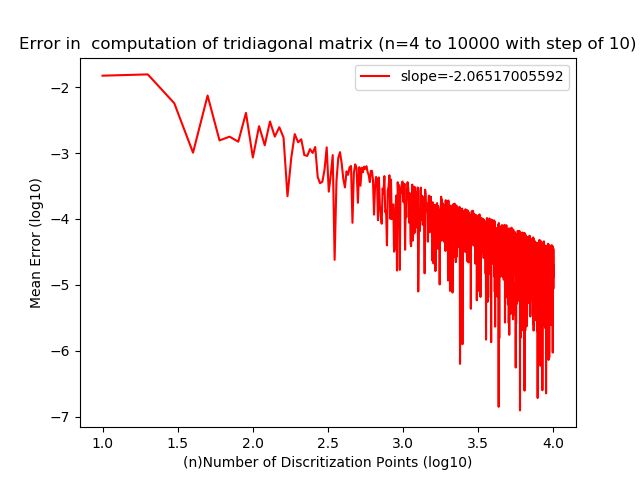
\includegraphics[width=0.7\linewidth]{data2_NPlog.png}
\caption{Normal scale with log computed plot of error in numerical computation of tridiagonal matrix (N=4 to 10000 with step of 10)}
\label{fig:data2_NPlog}
\end{figure}


\begin{figure}[!htbp]
\centering
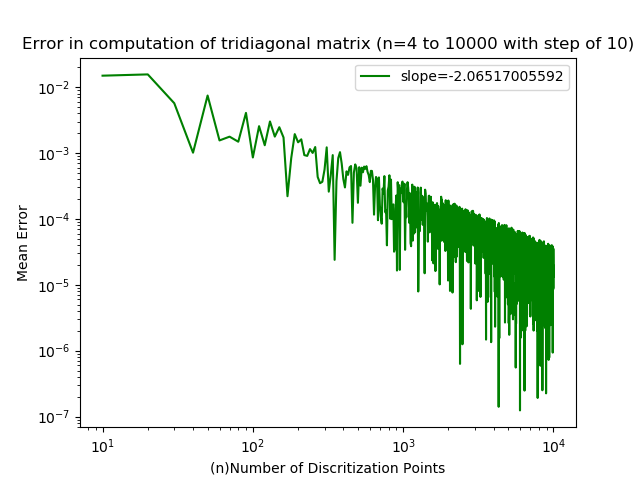
\includegraphics[width=0.7\linewidth]{data2_PLlog.png}
\caption{Log scale plot of error in numerical computation of tridiagonal matrix (N=4 to 10000 with step of 10)}
\label{fig:data2_PLlog}
\end{figure}



%% The Appendices part is started with the command \appendix;
%% appendix sections are then done as normal sections
%\appendix

%\section{Section in Appendix}
%\label{appendix-sec1}

%Sample text. Sample text. Sample text. Sample text. Sample text. Sample text. 
%Sample text. Sample text. Sample text. Sample text. Sample text. Sample text. 
%Sample text. 

%% References
%%
%% Following citation commands can be used in the body text:
%% Usage of \cite is as follows:
%%   \cite{key}         ==>>  [#]
%%   \cite[chap. 2]{key} ==>> [#, chap. 2]
%%

%% References with bibTeX database:

%\bibliographystyle{elsarticle-num}
% \bibliographystyle{elsarticle-harv}
% \bibliographystyle{elsarticle-num-names}
% \bibliographystyle{model1a-num-names}
% \bibliographystyle{model1b-num-names}
% \bibliographystyle{model1c-num-names}
% \bibliographystyle{model1-num-names}
% \bibliographystyle{model2-names}
% \bibliographystyle{model3a-num-names}
% \bibliographystyle{model3-num-names}
% \bibliographystyle{model4-names}
% \bibliographystyle{model5-names}
% \bibliographystyle{model6-num-names}

%\bibliography{sample}


\end{document}

%%
%% End of file
